\chapter{Θεωρία πληροφοριών}
\label{chapter:chap3}

\section{Εισαγωγή}
\label{section:sect31}

\indent Σε αυτό το κεφάλαιο γίνεται μια εισαγωγή σε βασικά στοιχεία της Θεωρίας πληροφοριών και κυρίως στην επεξήγηση της έννοιας εντροπία της πληροφορίας. Επίσης θα αναφερθούν αλγόριθμοι συμπίεσης (entropy encoding) καθώς και ο αλγόριθμος kmeans που χρησιμοποιήθηκε για την παραγωγή των codebooks.

\section{Εντροπία}
\label{section:sect32}

\indent Η εντροπία κατά Shannon που εισήχθηκε από τον Claude E. Shannon το 1948 είναι η ποσοτικοποίηση της αβεβαιότητας μιας τυχαίας μεταβλητής και συνήθως μετριέται σε bits η nats. Η κύρια πληροφορία που παρέχεται από την εντροπία και είναι χρήσιμη σε εμάς είναι το απόλυτο κάτω όριο οπού η πληροφορία μπορεί να συμπιεστεί. Η εντροπία ορίζεται ως $ H(X) = -\sum_{i=1}^{n} p(x_i)*\log_{b} p(x_i) $  οπού $p(x_i)$ είναι η πιθανότητα του ενδεχομένου $x_i$ και b είναι οι μονάδα μέτρησής της εντροπίας.Για συμπίεση δεδομένων συνήθως ισχύει $b=2$ έτσι ώστε να έχουμε την εντροπία σε bits.

\indent Για να κατανοήσουμε την εντροπία θα δοθεί ένα παράδειγμα. Έστω ότι πρέπει να αναπαρασταθεί σε δυαδικό σύστημα μια ακολουθία από αριθμούς $x_i \in [0,3] $. Επομένως υπάρχουν $n=4$ διαφορετικά ενδεχόμενα που χρειάζονται 2 bits το καθένα για να αναπαρασταθούν
$x_i = \begin{bmatrix}
0 & 0 \\
0 & 1 \\
1 & 0 \\
1 & 1
\end{bmatrix} $. Αν τα ενδεχόμενα είναι ισοπίθανα $ p(x_i)= 0.25 $ τότε έχουμε $ H(X) = 2bits $ άρα δε μπορούμε να κάνουμε κάτι για να τα συμπιέσουμε. Αν όμως είναι $ p(x_1) = 0.7, p(x_2)=p(x_3)=p(x_4)=0.1 $ τότε έχουμε $ H(X) = 1.35678 bits$ ανά σύμβολο κατά μέσο όρο. Επομένως τα δεδομένα μας μπορούν ιδανικά να συμπιεστούν κατά $(1-1.35678/2)\% = 32\%$.

\section{Κωδικοποιητές Εντροπίας}
\label{section:sect33}

\indent Οι μέθοδοι που σήμερα υπάρχουν για συμπίεση καταφέρνουν να έρθουν πολύ κοντά στο όριο που δίνει η εντροπία αλλά δε το φτάνουν. Δύο είναι οι κυρίαρχες, η μέθοδος Huffman και Αριθμητική κωδικοποίηση με την δεύτερη να είναι αυτή που χρησιμοποιείται περισσότερο στο βίντεο με την παραλλαγή της που λέγεται CABAC (Context Adaptive Binary Arithmetic Coding)
\begin{itemize}
  \item Η μέθοδος Huffman έχει την μικρότερη πολυπλοκότητα O(nlogn) και μας εξασφαλίζει πώς $ H(X) \leq HC \leq H(X)+1bit  $ όπου HC είναι το μέσο μήκος ανά σύμβολο που δίνει ο Huffman. Ο αλγόριθμος βάζει τα ενδεχόμενα σε ένα δυαδικό δέντρο και τους αναθέτει λέξεις με διαφορετικό μήκος με στοχο το ενδεχόμενο με την μεγαλύτερη πιθανότητα θα έχει το μικρότερο μήκος και αυτό με την μικρότερη πιθανότητα το μεγαλύτερο μήκος. Έστω λοιπόν ότι έχουμε 5 ενδεχόμενα $x_i$ με πιθανότητες $p(S_0) = 0.5, p(S_1)=p(S_2)=0.2, p(S_3)=p(S_4)=0.05$ το δέντρο Huffman για αυτό το παράδειγμα φαίνεται στο Σχήμα~\ref{fig:huffman}.
      \begin{figure}[h!]
          \centering
          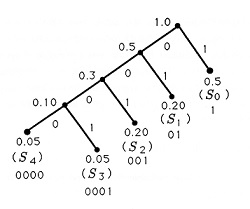
\includegraphics[width=0.5\textwidth]{chapter3/huffman.jpg}
          \caption{Δέντρο Huffman.}
          \label{fig:huffman}
      \end{figure}

\newpage
  \item Η μέθοδος της Αριθμητικής Κωδικοποίησης έχει την μεγαλύτερη πολυπλοκότητα αλλά μας εξασφαλίζει μια συμπίεση πού τις περισσότερες φορές είναι αρκετά καλύτερή από αυτή του Huffman και πλησιάζει αρκετά την εντροπία.Ο αλγόριθμος όπως και στον Huffman έχει στόχο να δώσει μεγάλο μήκος στα ενδεχόμενα με την μικρότερη πιθανότητα και μικρό σε αυτά με την μεγαλύτερη. Η διαφορά του με τον Ηuffman είναι πως δεν κωδικοποιεί ανά σύμβολο αλλά όλο την σειρά συμβόλων σε έναν μοναδικό αριθμό $n \in R$. Έστω μια κατανομή με 3 σύμβολα A,B,C και τις πιθανότητες τους $ p(A) = 0.5, p(B) = 0.33, p(C) = 0.17 $ και κωδικοποιείται το μήνυμα "BCA" . Στο Σχήμα~\ref{fig:ac} φαίνονται τα βήματα της κωδικοποίησης οπού στο πρώτο βήμα έρχεται το B και το κωδικοποιούμε με τον αριθμό 0b01(x) γιατί έχει το μικρότερο μήκος και βρίσκεται στο [0.5,0.83) οπού x σημαίνει αυθαίρετη ακολουθία από bits. Έτσι σύνεχίζουν και τα υπόλοιπα βήματα μέχρι να έχουμε τον αριθμό που αντιστοιχεί στην ακολουθία.

      \begin{figure}[ht!]
          \centering
          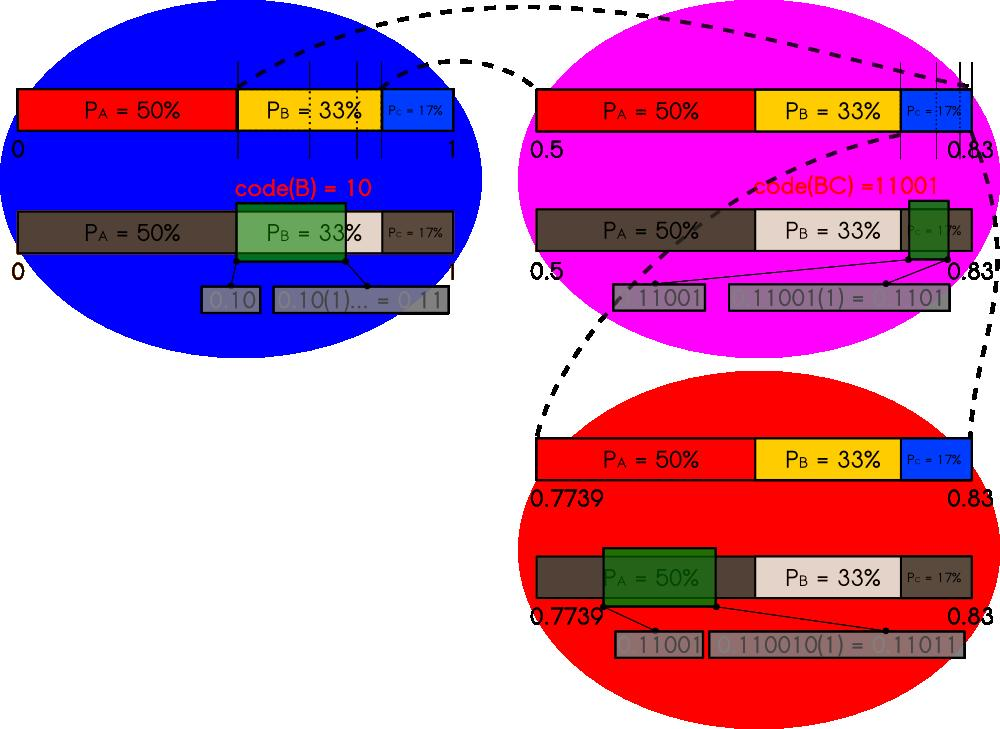
\includegraphics[width=0.5\textwidth]{chapter3/ac.jpg}
          \caption{Βήματα αριθμητικής κωδικοποίησης.}
          \label{fig:ac}
      \end{figure}
\end{itemize}

\newpage
\section{Αλγόριθμος clustering kmeans}
\label{section:sect34}

\indent Άλλο ένα στοιχείο που χρησιμοποιήθηκε σε αυτή την διπλωματική και πηγάζει από την Θεωρία πληροφοριών είναι ο αλγόριθμος clustering kmeans. Είναι ένας επαναληπτικός αλγόριθμος όπου στόχος του είναι να χωρίσει με το ελάχιστο σφάλμα n σημεία με διάσταση d σε k περιοχές $ k \leq n $ όπως φαίνεται στο Σχήμα~\ref{fig:kmeans}. O kmeans έχει πολύ μεγάλη υπολογιστική πολυπλοκότητα και ανάγεται στα προβλήματα NP-hard. Παρακάτω δίνετε σε ψευδοκώδικα ο αλγόριθμος.\\

\begin{algorithmic}[1]
\STATE{Choose initial centers for clusters K;}
\WHILE{the clusters are changing}
    \STATE{Reassign the data points and set $Ktemp=0$;}
    \FORALL{Data points n}
        \STATE{Assign data point $n_i$ to the cluster $k_j$ whose center is closest;}
        \STATE{$Ktemp_j+=n_i$}
    \ENDFOR
    \STATE{Update the cluster centers;}
    \FOR{j:=1 to k step 1}
        \STATE{$\mathbf{r_j}$ = number of points in $Ktemp_j$;}
        \STATE{$\mathbf{K_j} = \frac{Ktemp_j}{r_j}$;}
    \ENDFOR
\ENDWHILE
\end{algorithmic}

\begin{figure}[ht!]
  \centering
  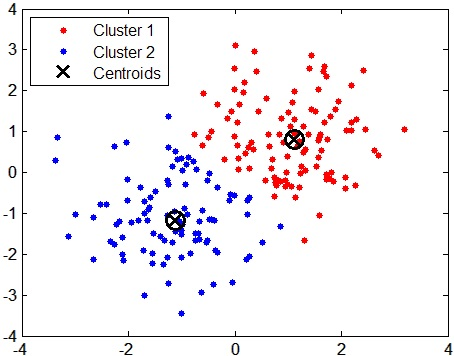
\includegraphics[width=0.5\textwidth]{chapter3/kmeans.jpg}
  \caption{kmeans με $k=2,d=2,n=100,MSE=284.671$}
  \label{fig:kmeans}
\end{figure}

\newpage

\indent Στο Βημα 1 του kmeans γίνετε η αρχικοποίηση στην οποία μπορούμε να επιλέξουμε να είναι τυχαία (δηλαδή κάθε cluster να παίρνει τιμές από ένα τυχαίο point) η να έχουμε κάποια στρατηγική. Στην παρούσα διπλωματική επιλέχθηκε να η στρατηγική KKZ (Katsavounidis Kuo Zhang) η οποία είναι πιο αργή από την τυχαία αλλά ο kmeans συγκλίνει πιο γρήγορα και σε καλύτερο σφάλμα. Ο αλγόριθμος παραλληλοποιήθηκε και επιτεύχθηκε γραμμική επιτάχυνση δοκιμασμένο 1,2,4,8,12,24 νήματα. Στο Σχήμα ~\ref{fig:kkzspeed} φαίνεται η επιτάχυνση του παράλληλου αλγορίθμου και στο Σχήμα ~\ref{fig:kkziter} φαίνονται οι συνολικές επαναλήψεις που κάνει ο kmeans με τυχαία και KKZ αρχικοποίηση.

\begin{figure}[ht!]
  \centering
  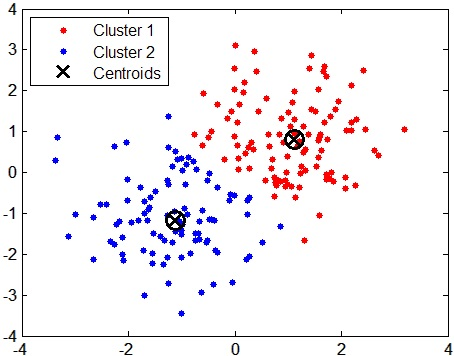
\includegraphics[width=0.5\textwidth]{chapter3/kmeans.jpg}
  \caption{kmeans με $k=2,d=2,n=100,MSE=284.671$}
  \label{fig:kkzspeed}
\end{figure}

\begin{figure}[ht!]
  \centering
  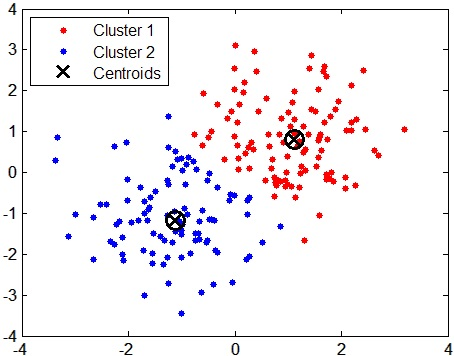
\includegraphics[width=0.5\textwidth]{chapter3/kmeans.jpg}
  \caption{kmeans με $k=2,d=2,n=100,MSE=284.671$}
  \label{fig:kkziter}
\end{figure}

\newpage

\indent Η πιο σημαντική βελτιστοποίηση επιτεύχθηκε στο σημείο της αναζήτησης του κοντινότερου cluster στο Βήμα 5. Στην απλή εκδοχή του αλγορίθμου για κάθε data point σαρώνονται όλα τα clusters για να βρεθεί ποιο είναι πιο κοντά. Στην διπλωματική αυτή χρησιμοποιήθηκε ο αλγόριθμος Fast Nearest Neighbour οπού οργανώνει τις αποστάσεις σε ένα δυαδικό δέντρο και μας επιτρέπει να κάνουμε από k αναζητήσεις log(k) για κάθε data point. Αυτό δίνει μία τεράστια επιτάχυνση στο όλο πρόβλημα και σε συνδυασμό με την παραλληλοποίηση του Βήματος 4 μας επέτρεψε να τρέχουμε μεγάλα πειράματα σε εύλογο χρονικό διάστημα. Οι επιταχύνσεις που επιτεύχθηκαν με την χρήση του FastNN φαίνεται στο Σχήμα~\ref{fig:fastnn} και της παραλληλοποίησης του Βήματος 4 στο Σχήμα~\ref{fig:ompiter}

\begin{figure}[ht!]
  \centering
  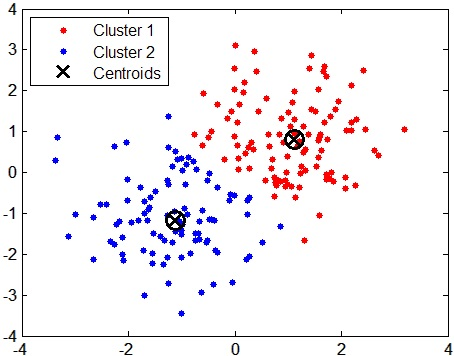
\includegraphics[width=0.5\textwidth]{chapter3/kmeans.jpg}
  \caption{kmeans με $k=2,d=2,n=100,MSE=284.671$}
  \label{fig:fastnn}
\end{figure}

\begin{figure}[ht!]
  \centering
  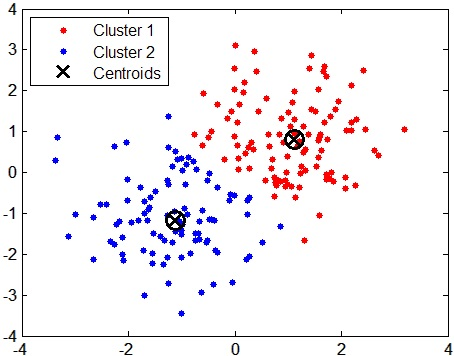
\includegraphics[width=0.5\textwidth]{chapter3/kmeans.jpg}
  \caption{kmeans με $k=2,d=2,n=100,MSE=284.671$}
  \label{fig:ompiter}
\end{figure}

\newpage
\indent Για τα πειράματα της διπλωματικής χρησιμοποιήθηκε ένας HP Blade Server
\begin{itemize}
    \item OS Microsoft Windows Server 2008 R2 Datacenter.
    \item CPU 2xIntel Xeon E5-2600 @ 2.30Ghz οπού παρείχαν συνολικά 12 Threads + 12 με HyperThreading.
    \item RAM 32GB.
\end{itemize} 